\chapter{Continuous-Time Identification}

We start this discussion considering LTI SISO models.\\

The problem involves finding the parameters \(\theta\) of a model of the form:
\[
H(s, \theta) = \frac{\beta_{n-1}s^{n-1} + \beta_{n-2}s^{n-2} + \cdots + \beta_1s + \beta_0}{s^n + \alpha_{n-1}s^{n-1} + \alpha_{n-2}s^{n-2} + \cdots + \alpha_1s + \alpha_0}
\]
where
\[
\theta = [\alpha_1, \alpha_2, \ldots, \alpha_{n-1}, \beta_0, \ldots, \beta_{n-1}]
\]

This problem needs to be solved using noisy and sampled data. The block diagram scheme for this problem is shown below:

\begin{figure}[htbp]
    \centering
    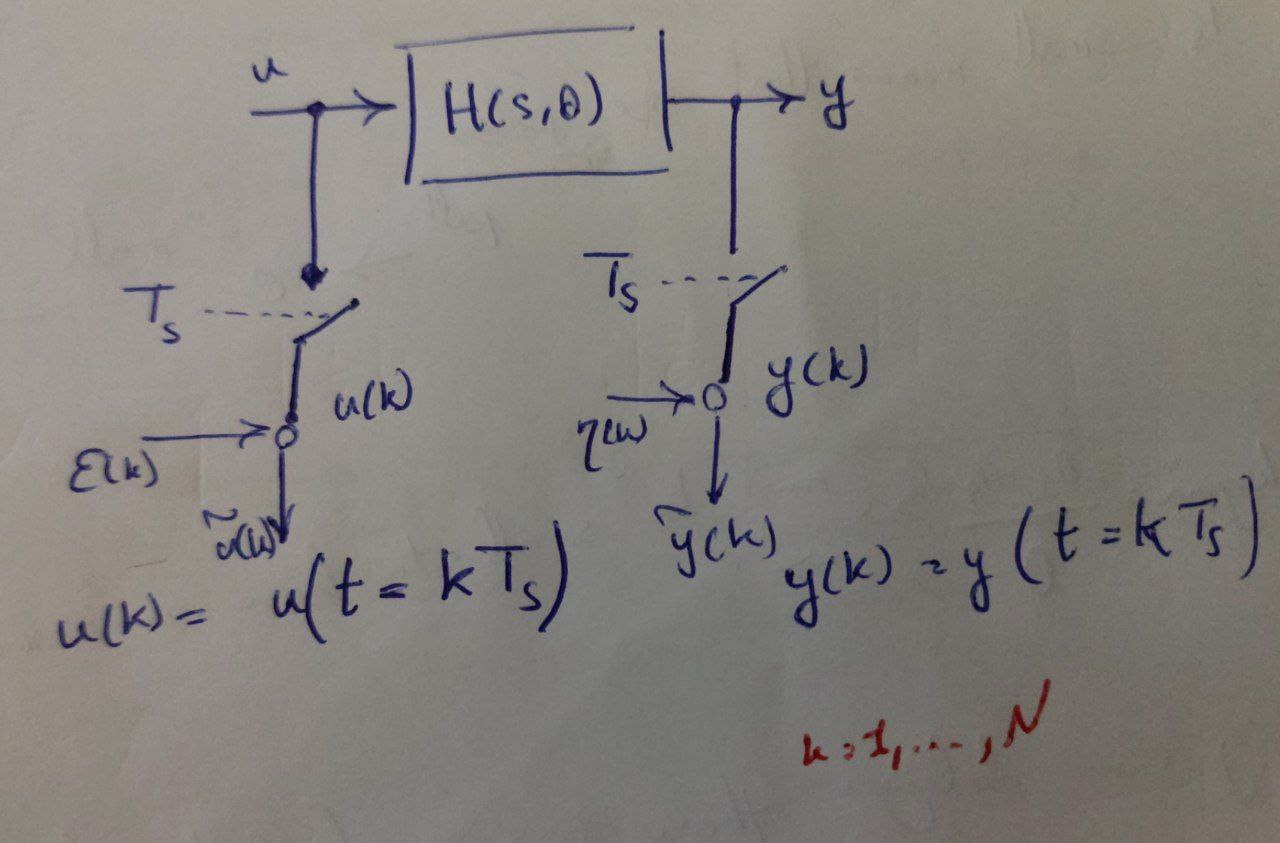
\includegraphics[width=0.7\textwidth]{images/continuous-scheme.jpg}
    \caption{Block diagram representation of sampling data in the continuous scheme.}
    \label{fig:signal-and-noise}
\end{figure}

\textbf{Motivations:}
\begin{enumerate}
    \item By nature, the parameter vector \(\theta\) does not depend on the sampling rate \(T_s\).\\
    When \(T_s\) decreases, all the poles tend to 1. In particular, the poles of a DT system obtained by discretization of a continuous-time system are:
    \[
    P_{dt} = e^{-P_{ct}T_s}
    \]
    Consequently, to maintain a bounded DC gain, the parameters of the numerator tend to zero.

    \item Continuous-time models are closer to the physical description of systems.

    \item Most robust control design techniques are formulated in continuous-time, e.g., \(H_\infty\) and \(\mu\)-synthesis.
\end{enumerate}

\textbf{Two Families of Approaches for System Identification in This Domain:}
\begin{enumerate}
    \item \textbf{Indirect approach:}\\
    
    \begin{itemize}
        \item Estimate a discrete-time model from data.
        \item Use an inverse discretization method to transform this model into continuous-time:
        \[
        u(k) \xrightarrow{\text{Standard discrete identification}} H(q^{-1}, \theta) \xrightarrow{\text{Inverse discretization}} H(s, \theta_c)
        \]
    \end{itemize}
    This approach is simple but has some issues:
    \begin{itemize}
        \item It is not true continuous-time identification. This approach does not solve issues related to the choice of the sampling rate.
        \item Inverse discretization methods, in general, do not preserve important system properties such as stability.
    \end{itemize}

\begin{example}[MATLAB Code]
\begin{verbatim}
theta_LS = A\B; % LS estimation for the DT model
H_z = tf(theta_LS, theta_LS, T_s); % DT model transfer function
H_s = d2c(H_z, 'method'); % Convert to CT model
\end{verbatim}

For the method, you can use \texttt{'zoh'}. Note that the continuous-time parameters will be correct if the following conditions hold:

\begin{enumerate}
    \item The discrete-time parameters are accurate.
    \item \(u(t)\) remains constant over each time interval \([k, k+T_s]\), meaning the sampling rate is much faster than the dynamics of the actuator, look at the following figure.
\end{enumerate}

Another method is \textit{matched} which does the following:
\[
p^{ct} = \frac{\ln(p^{dt})}{T_s}
\]
\end{example}

\begin{figure}
    \centering
    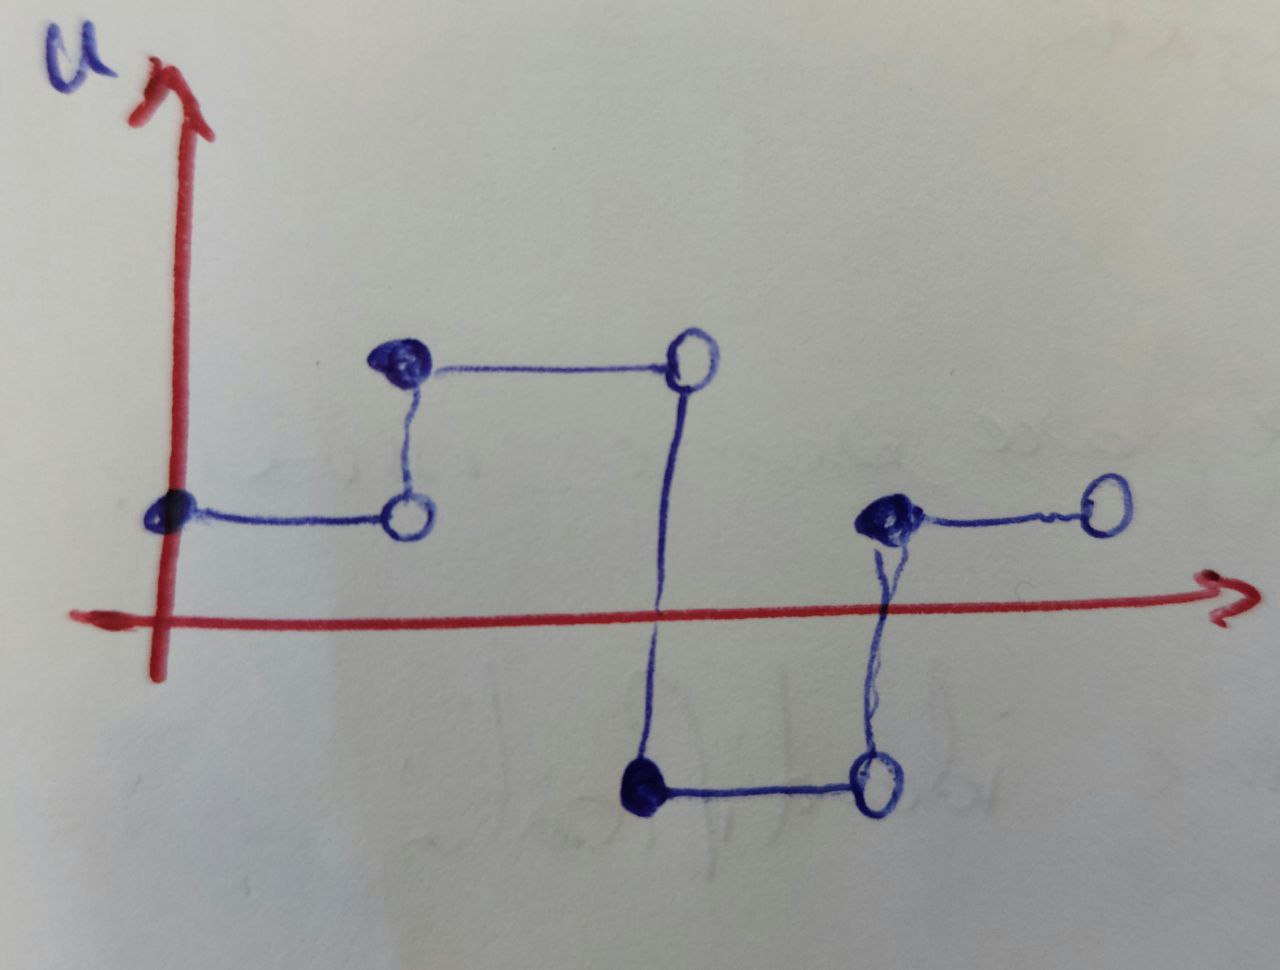
\includegraphics[width=0.35\textwidth]{images/discretized-input.jpg}
    \caption{A discretized input; notice that the value of \( u \) remains constant between consecutive sampling instances.}
\end{figure}
\newpage
    \item \textbf{Direct approach}\\
    
Let us consider a simple example:
\[
H(s) = \frac{\beta_0 + \beta_1s}{s + \alpha_0}
\]
\[
y(s) = H(s) u(s)
\]
Considering zero initial condition for our system:
\[
s y(s) + \alpha_0 y(s) = \beta_1 s u(s) + \beta_0 u(s)
\]
\[
\xrightarrow{\mathcal{L}^{-1}} \dot{y}(t) + \alpha_0 y(t) = \beta_1 \dot{u}(t) + \beta_0 u(t)
\]
Notice that if we could measure $\dot{y}(t)$ and $\dot{u}(t)$, by taking sampled measurements. We could use LS in order to solve the problem, by shaping the regression matrix and output matrix.


\subsubsection{How to obtain $\dot{y}(k)$ and $\dot{u}(t)$ }
We cannot use a derivative block, since it is anti-causal, the best case is implementing a high-pass filter, but we know that a high-pass filter amplifies the noise.\\

We try to estimate them:
\[
\dot{y}(t) = D(q^{-1})y(k)
\]
where $D$ is some discretization of $H(s) = s$.\\

This is a numerical derivative method. The problem is that we need to do this using measured output samples. Therefore, if the measurements have high-freuqnecy components, or at any rate noise, they would be amplified.
\[
\dot{y}(k) = D(q^{-1})y(k) +D(q^{-1})\eta(k)
\]

Another important aspect to take into consideration is that, in this method, the noises becomes correlated, even if the original noise samples are not correlated, and for this reason we cannot employ Least Squared method.\\

\textbf{Instead we try to estimate the following signals:}
\[
y^{I}(t) = \mathcal{L}^{-1}\{Y^{I}(s)\} \:\:\text{ where }\:\: Y^{I}(s) = \lambda(s) Y(s)
\]
\[
u^{I}(t) = \mathcal{L}^{-1}\{U^{I}(s)\} \:\:\text{ where }\:\: U^{I}(s) = \lambda(s) U(s)
\]
where, $lambda$ is a low-pass filter, which is a linear dynamic operator.
\[
\lambda(s) = \frac{1}{1 + s\tau}
\]
in which $\tau$ is a user-choice time-constant.\\

Therefore,
\[
s(\lambda) = \frac{1 - \lambda}{\lambda\tau}
\]
By substituting the last statement in our equation we obtain:
\[
\frac{1-\lambda}{\lambda\tau}y + \alpha_0y = \beta_1\frac{1 - \lambda}{\lambda\tau} u +\beta_0 u
\]
\[
(1-\lambda)y + \alpha_0\lambda\tau y = \beta_1(1 - \lambda) u +\beta_0\lambda\tau u
\]
\[
y = (1-\alpha_0 \tau)\lambda y + \beta_1 u + (\beta_0 \tau - \beta_1) \lambda u
\]
Now, we need to come back to time; in the sense that:
\[
u(\lambda) \rightarrow u(t)
\]
\[
y(\lambda) \rightarrow y(t)
\]
Here, the arrow represents two sequence, 
\begin{enumerate}
    \item replace $\lambda$ with $\lambda(s)$
    \item inverse Laplace transform
\end{enumerate}

\[
y(t) = (1-\alpha_0 \tau)y^{(I)}(t) + \beta_1 u(t) + (\beta_0 \tau - \beta_1) u^{(I)}(t)
\]

taking \(t = kT_s\) for \(K = 1,\,2,\,\cdots,\,N\) measurements, and considering the following naming for our parameters, we obtain:
\[
\begin{bmatrix}
\gamma_1 \\
\gamma_2 \\
\gamma_3
\end{bmatrix}
=
\begin{bmatrix}
(1 - \alpha_0 \tau) \\
\beta_1 \\
(\beta_0 \tau - \beta_1)
\end{bmatrix}
\]

\[
\begin{bmatrix}
y(1) \\
y(2) \\
\cdots \\
y(N)
\end{bmatrix}
= \begin{bmatrix}
y^{(I)}(1) & u(1) & u^{(I)}(1) \\
y^{(I)}(2) & u(2) & u^{(I)}(2) \\
\vdots & \vdots & \vdots \\
y^{(I)}(N) & u(N) & u^{(I)}(N)
\end{bmatrix}
\begin{bmatrix}
\gamma_1 \\
\gamma_2 \\
\gamma_3
\end{bmatrix}
\]
$\gamma$s are the parameters of the transformed model, which is the model relating $u$, and $y$ with $\lambda$. \\

The signals $y^{(I)}$ and $u^{(I)}$ are obtained by simulating without amplifying the noise! \\

Finally,
\[
\begin{bmatrix}
\gamma_1 \\
\gamma_2 \\
\gamma_3
\end{bmatrix}
=
\begin{bmatrix}
-\tau & 0 & 0 \\
0 & 0 & 1 \\
0 & \tau & -1
\end{bmatrix}
\begin{bmatrix}
\alpha_1 \\
\beta_0 \\
\beta_1
\end{bmatrix}
+
\begin{bmatrix}
1 \\
0 \\
0
\end{bmatrix}
\]
\end{enumerate}

\section{Set-membership identification of continuous-time systems}
A-priori information on the system:

\[
H(s, \theta) = \frac{\beta_{n-1}s^{n-1} + \beta_{n-2}s^{n-2} + \cdots + \beta_1s + \beta_0}{s^n + \alpha_{n-1}s^{n-1} + \alpha_{n-2}s^{n-2} + \cdots + \alpha_1s + \alpha_0}
\]

A-priori information on the noise: sampled EIV data.
\[
\tilde{y}(k) = y(k T_s) + \eta(k)\]
\[
\tilde{u}(k) = u(k T_s) + \xi(k)
\]
and 
\[
|\eta(.)| \leq \Delta\eta
\]
\[
|\xi(.)| \leq \Delta\xi
\]

There are two SM approaches to solve this problem:
\begin{enumerate}
    \item based on model transformation 
    \item based on Tustin discretization
\end{enumerate}

\subsection{Tustin Discretization}
Consider an integrator with the following transfer function:
\[
H(s) = \frac{1}{s}
\]
We know that in the time domain, this system act as follows:
\[
y(t) = y(t_0) + \int_{0}^{t} u(\tau)d\tau
\]
know, consider that this continuous-time function is sampled at $t = k T_s$ to $(k+1) T_s$, which can be rewritten in this way:
\[
y(k+1) = y(k) + \int_{K T_s}^{(k+1)T_s} u(\tau)d\tau
\]
and the method used for \textbf{the integration is trapsoidal}. After all, we should have an assuption about how the function behave between the sample times to be able to perform the integration, so the area becomes:
\[
\frac{(u(k+1) + u(k))}{2}T_s
\]
\begin{factbox}
Then, having this assumption, it can be understood that the identification improves as:
\begin{enumerate}
    \item as $T_s$ gets smaller
    \item applying smooth signals such as multi-sin signlas.
\end{enumerate}
\end{factbox}
and as a result,
\[
y(k+1) = y(k) + \frac{(u(k+1) + u(k))}{2}T_s
\]

Now, considering the time-shift operator, the equation can be written in the following form:
\[
(q-1) y(k) = \frac{Ts}{2}(1+q)u(k)
\]
\[
H(q) = \frac{y(k)}{u(k)} = \frac{Ts}{2} \frac{q+1}{q-1}
\]
This is Tusting discretization of the $\frac{1}{s}$. In general we replace $s$ by:
\[
s \rightarrow \frac{2}{T_s}\frac{z-1}{z+1}
\]

Back to our set-membership identification of continuous-time systems, let's consider:
\[
H(s) = \frac{\beta_1 s + \beta_0}{s^2 + \alpha_1 s + \alpha_0 }
\]
where after performing Tustin discritization it becomes;
\[
H(z) = \frac{\beta_1 \frac{2}{T_s}\frac{z-1}{z+1}+ \beta_0}{(\frac{2}{T_s}\frac{z-1}{z+1})^2 + \alpha_1 (\frac{2}{T_s}\frac{z-1}{z+1}) + \alpha_0}
\]

\begin{figure}[htbp] 
    \centering
    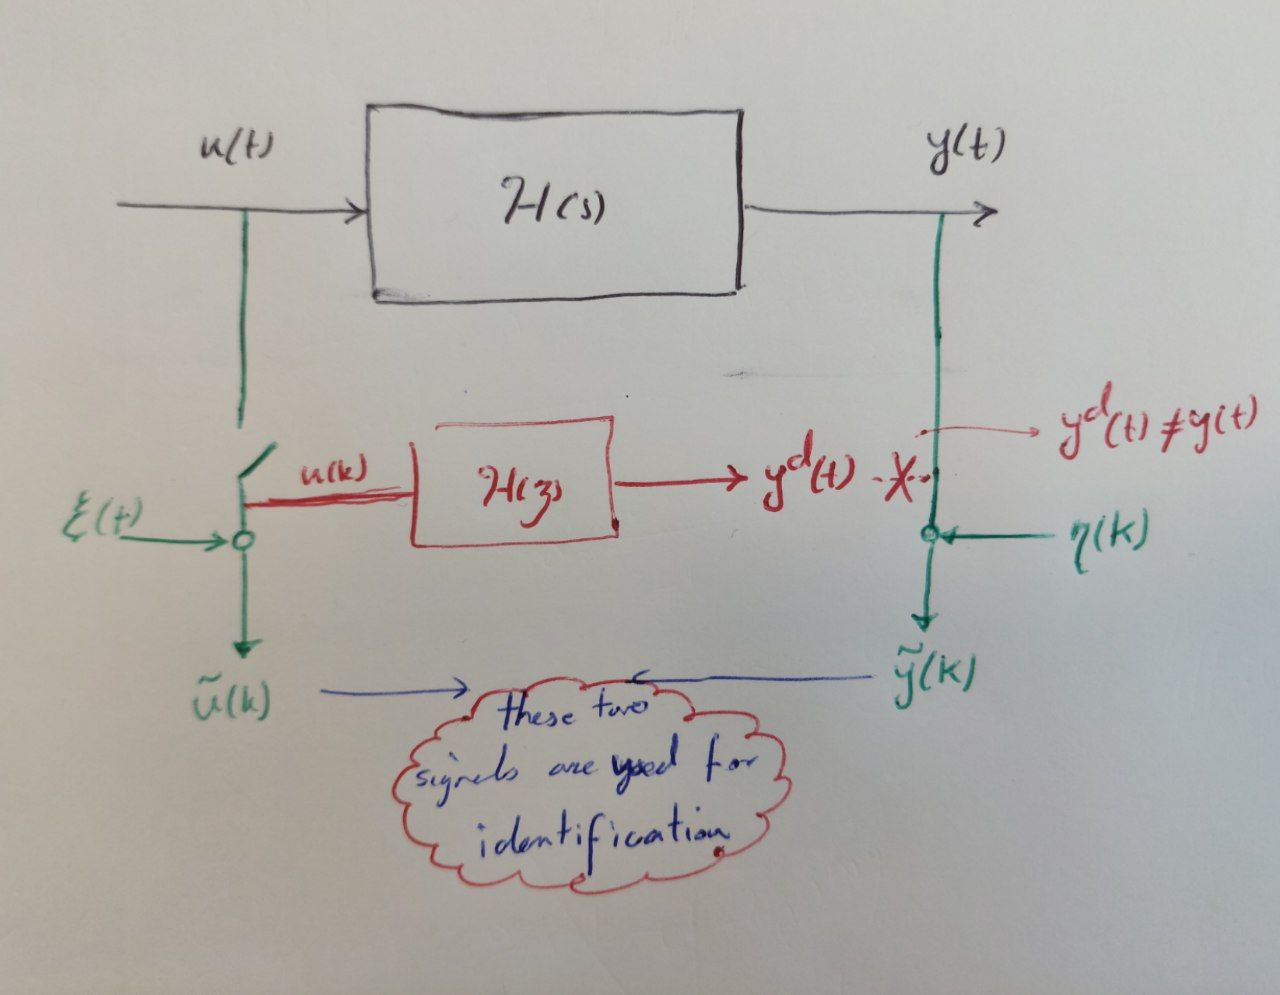
\includegraphics[width=0.75\textwidth]{images/tustin-discritization.jpg}
    \caption{scheme of the Tustin discretization set-membership identification of the continuous-time systems}
    \label{fig:FPS_time_domain}
\end{figure}

Here, 
\[
y^d(k) = H^{Tustin}(q^{-1})u(k) \neq y(k) = y(k T_s)
\]

if the assumption required by the discretization are not perfectly met.

We define
\[
\delta(k) = y^d(k) - y(k)
\]
according to set-membership framework, and we consider it as another a-priori assumption. The same as the assumption on the bound of the noise:
\[
|\delta(k)|\leq \Delta\delta
\]
\[
\begin{cases}
\delta(k) = y^d(k)-y(k)\\
\tilde{y}(k) = y(k) + \eta(k)
\end{cases}
\Rightarrow
\delta(k) = y^d(k) + \eta(k) - \tilde{y}(k)
\]
Now we introduce another component:
\[
\eta^{'}(k) \leq \Delta \eta + \Delta \delta
\]
Pay attention that $\Delta \delta$ tends to zero as $T_s \to 0$.\\
Having defined $\delta$, we can solve the problem dealing with less data, thereby solving the problem in a considerably shorter time. 

\subsubsection{Defining feasible parametric set}
\[
\mathcal{D}_\theta = \left\{ \theta \in \mathbb{R}^4 : 
\begin{aligned}
H(s) &= \frac{\beta_1 s + \beta_0}{s^2 + \alpha_1 s + \alpha_0 }, \\
\tilde{y}(k) &= y^d(k) + \eta^{'} , \quad |\eta^{'}| \leq \Delta\eta + \Delta\delta, \\
\tilde{u}(k) &= u(k) + \zeta^{'} , \quad |\zeta^{'}| \leq \Delta\zeta , \\
y^d(k) &= H(z) u(k), \quad \forall k = 1,\, 2,\, \dots,\, N
\end{aligned}
\right\}
\]

Now, we simplify $H(z)$ by multiplicating and divinding it by $Ts (z+1)^2$,
\[
H(z) = \frac{2 Ts (z+1) \beta_1(z-1) + T_s^2 (z+1)^2\beta_0 )}{4(z-1)^2 + 2\alpha_1 T_s(z-1)(z+1) + T_S^2(z+1)^2\alpha_0}
\]

\[
H(z) = \frac{2 T_S (z^2-1) +T_s^2 (z+1)^2 \beta_0}{4(z^2-2z+1) + 2\alpha_1 T_s (z^2-1) + T_s^2 \alpha_0 (z^2 + 2z + 1)}
\]

\[
H(z) = \frac{z^2(2T_s \beta_1 + T_s^2\beta_0) + z(2 T_s \beta_0) + T_s^2 \beta_1 - 2 T_s \beta_1}{z^2(4 + 2 \alpha_1 T_s + \alpha_0 T_s^2) + z(-8 + 2 T_s^2 \alpha_0) + 4 - 2 \alpha_1 T_s + T_s^2 \alpha_0}
\]

We want to reconduce the form:
\[
H(z) = \frac{\zeta_2 z^2 + \zeta_1 z + T_s^2 \zeta_0}{z^2 + \gamma_1 z +  \gamma_0}
\]

Pay attention that, in order to obtain a unique transfer function, the coefficient of the largest term in the denumerator of the transfer function should be 1. Therefore, we divide and multipli the transfer function, by the coefficient of $z^2$ in the denumerator, which is name as $a_2$, the coefficient of numerator are called $b$.\\

Now, we define the extended parameter set.

\[
\mathcal{D}_{\theta,\,\zeta,\,\gamma,\,\eta,\,\xi} = \left\{ \theta \in \mathbb{R}^4,\, \zeta \in \mathbb{R}^3,\,\gamma \in \mathbb{R}^2,\,\xi,\,\eta^{'} \in \mathbb{R}^N,\, : 
\begin{aligned}
\tilde{y}(k) &= y^d(k) + \eta^{'} , \quad |\eta^{'}| \leq \Delta\eta + \Delta\delta, \\
\tilde{u}(k) &= u(k) + \zeta^{'} , \quad |\zeta^{'}| \leq \Delta\zeta , \\
y^d(k) &= H(q^{-1},\zeta,\,\xi) u(k), \quad \forall k = 1,\, 2,\, \dots,\, N \\
\zeta_i a_2(\alpha) &= b_i(\beta), i = 0,\, 1,\,2\\
\gamma_i a_2(\alpha) &= a_i(\alpha) i = 0,\,1
\end{aligned}
\right\}
\]
The third equation is writen in implecite form to save some space, this equation should be considered in the following form:
\[
y^d(k) + \gamma_1 y^d(k-1) + \gamma_2 y^d(k-2) = \zeta_2 u(k) + \zeta_1 u(k-1) + \zeta_0 u(k-2)
\]
and considering the noise-corrupted data samples at hand:
\[
\begin{array}{c}
\tilde{y}(k) - \eta^{'}(k) + \gamma_1\tilde{y}(k-1) - \eta^{'}(k-1) + \gamma_2 \tilde{y}(k-2) - \eta^{'}(k-2) = \\ \zeta_2 \tilde{u}(k) - \zeta_2 \xi(k) +\zeta_1 \tilde{u}(k-1) - \zeta_1 \xi(k-1) + \zeta_0 \tilde{u}(k-2) - \zeta_0 \xi(k-2)
\end{array}
\]

\[
\underline{\theta}_i = \arg \min_{\substack{(\theta, \gamma, \xi, \eta', \zeta) \\ \in \mathcal{D}_{\theta, \gamma, \xi, \eta', \zeta}}} \theta_i
\]

\[
\overline{\theta}_i = \arg \min_{\substack{(\theta, \gamma, \xi, \eta', \zeta) \\ \in \mathcal{D}_{\theta, \gamma, \xi, \eta', \zeta}}} -\theta_i
\]

Finally, we recognize that $\zeta_i a_2(\alpha)$ and $\gamma_i a_2(\alpha)$ are in $\theta,\,\zeta,\,\gamma$ and the problem of computing PUI on $\alpha,\,\beta$ is a POP.

\subsubsection{Remarks about this approach}
\begin{itemize}
    \item If we assumed $\Delta\delta = 0$ and we use noise-free data; then, the problems of finding the PUIs might become \textbf{infeasible}, due to assuming a strong a-priori assumption.
    \item Notice that \textbf{the bound on the discretization error} must be provided as an a-priori assumption, but \textbf{it depends on the sampling rate $T_s$ and on the input signal.}\\
    a possibility is to estimate $\Delta\delta$ from the available data as follows: we try to solve the following problem until we obtain a feasible solution:\\
    \[
    \Delta^{*}_\delta = \arg \min \Delta_\delta \text{  s.t  } 
    \begin{aligned}
\tilde{y}(k) &= y^d(k) + \eta^{'} , \quad |\eta^{'}| \leq \Delta\eta + \Delta\delta, \\
\tilde{u}(k) &= u(k) + \zeta^{'} , \quad |\zeta^{'}| \leq \Delta\zeta , \\
y^d(k) &= H(q^{-1},\zeta,\,\xi) u(k), \quad \forall k = 1,\, 2,\, \dots,\, N \\
\zeta_i a_2(\alpha) &= b_i(\beta), i = 0,\, 1,\,2\\
\gamma_i a_2(\alpha) &= a_i(\alpha) i = 0,\,1
\end{aligned}
    \]
    However, there is no guaranatee that $\Delta_\delta^{*}$ will  be larger than the true bound on the discretization error. 
\end{itemize}





